%%%%%%%%%%%%%%%%%%%%%%%%%%%%%%%%%%%%%%%%%%%%%%%%%%%%%%%%%%%%%%%%%%%%
%           Auteur :  P.TRAN BA, E.BOUTTIER, J.SHI, E.ABIA         %
%         Création :  18/01/2012 17:05                             %
%%%%%%%%%%%%%%%%%%%%%%%%%%%%%%%%%%%%%%%%%%%%%%%%%%%%%%%%%%%%%%%%%%%%

\documentclass[a4paper,11pt]{article}

%\usepackage[utf8]{inputenc}
%\usepackage[T1]{fontenc}
%\usepackage{xunicode}
\usepackage{fontspec}
\defaultfontfeatures{Mapping=tex-text,Scale=MatchLowercase}
\usepackage{a4wide}
\usepackage{verbatim}
\usepackage{polyglossia}
\setdefaultlanguage{french}
%~ \usepackage{listings}
%\usepackage[french]{babel}
%~ \usepackage{url}
%~ \usepackage{times}
\usepackage{minted}
\usepackage{graphicx}
% graphviz.tex
% originally written by Derek Rayside, November 2003
% following an idea that Daniel Jackson implemented in his Tagger program
%
% parameters to \digraph:
% 1 - parameters for \includegraphics (optional; default value is "scale=1")
% 2 - name of the digraph
% 3 - body of the digraph

\newcommand{\digraph}[3][scale=1]{
    \newwrite\dotfile
    \immediate\openout\dotfile=#2.dot
    \immediate\write\dotfile{digraph #2 {\string#3}}
    \immediate\closeout\dotfile
    \IfFileExists{#2.ps}
        % the postscript exists: include it
        { \includegraphics[#1]{#2} }
        % the postscript doesn't exist: tell the user how to create it
        { \fbox{ \begin{tabular}{l}
            The file \texttt{#2.ps} hasn't been created from
            \texttt{#2.dot} yet. \\
            Run `\texttt{dot -Tps -o #2.ps #2.dot}' to create it. \\
            Here is a \textsf{bash} loop to process all \textsf{dot} files
            in the current directory: \\
            \texttt{
            for f in *.dot do ; 
            dot -Tps -o \$\{f\%dot\}ps \$f ; 
            done
            }
            \end{tabular}}
        }
}



\usepackage{geometry}
\geometry{hmargin=2.5cm,vmargin=1.5cm}

\title{Projet C : Simulation d'un commutateur de niveau 3\\Rapport}
\author{P.TRAN BA, E.BOUTTIER, J.SHI, E.ABIA\\Groupe 15}
\date\today

\begin{document}

\maketitle

\begin{abstract}

Ce rapport porte sur un projet de programmation d'un commutateur de niveau 3 en langage C. Il y est abordé le fonctionnement global du programme, suivi des choix techniques effectués afin de palier aux problèmes rencontrés. Il termine par une conclusion sur l'état du projet et des améliorations qui pourraient y être apportées.

\end{abstract}

\tableofcontents

\newpage

\section{Introduction}
\subsection{Préface}

Dans le cadre de notre préparation au diplôme d'ingénieur en Télécommunications et Réseaux, nous avons été amenés à effectuer notre projet de première année sous l’encadrement de Jérôme Ermont. Le but de ce projet était surtout de nous faire manipuler le langage C et la gestion de la mémoire mais il nous a permis de modéliser une solution réseau simple.

La commutation de paquets, technique utilisée dans le transfert de données dans les réseaux informatiques, permet de gagner du temps par la simultanéité de réception et de transfert de paquets différents. Il est donc intéressant de l’étudier. 

Ainsi il s’agissait dans ce projet de simuler le travail d’un élément réseau fictif dont le rôle serait de recevoir des trames, de les assembler pour former des paquets et d’effectuer par la suite la commutation de ces paquets. Il serait chargé ensuite d’envoyer les paquets routés à un élément en charge de la fragmentation et de l’ordonnancement des trames.

Comment répondre au cahier des charges tout en optimisant la mémoire ? 

Nous y répondrons en trois parties. La première partie présente l’application exécutable dans sa globalité, son fonctionnement. La seconde partie est consacrée au détail de l’implémentation. Enfin la troisième partie détaille la façon dont notre programme a été mis en œuvre.

\subsection{Rappel du sujet}

Il nous est demandé dans ce sujet de simuler le travail d’un élément réseau imaginaire, qui recevrait des trames (niveau 2, L-PDU), les assemblerait pour former des paquets (niveau 3, N-PDU), effectuerait ensuite la commutation, puis enverrait à un élément chargé de la fragmentation et de l’ordonnancement des trames. Nous allons présenter au fur et à mesure le fonctionnement de ces différents composants, et la simulation que l'on nous demande d’en faire.



% 
% \newpage
% \hspace{-3cm}
% 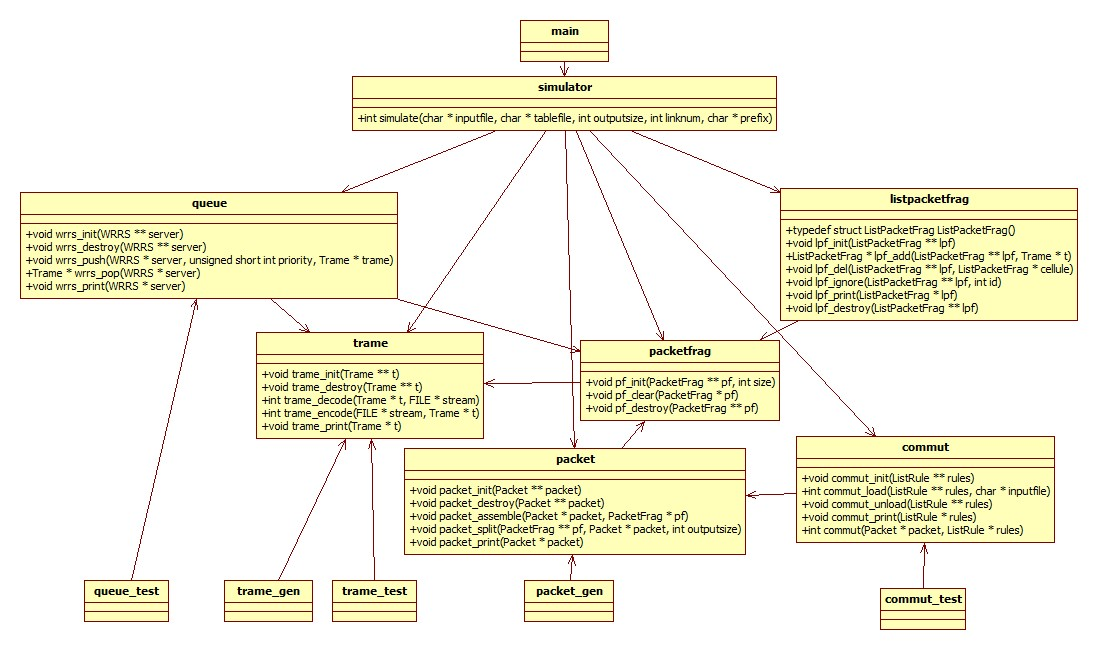
\includegraphics[width=18cm]{uml.pdf}
% \newpage
% 
% \subsection{Récupération des options}
% La classe Options possède des arguments public et static, correspondant
% aux différentes variables paramétrables.
% \begin{minted}[linenos,tabsize=4]{java}
% public static int typographie = 0; // Typographie d'affichage
% public static boolean couleur = false; // Affichage de la couleur
% public static boolean details = true; // Affichage du details de la solution
% public static int minimum = 0; // Longueur minimum de la solution
% public static int largeur = 20; // Largeur du labyrinthe
% public static int hauteur = 12; // Hauteur du labyrinthe
% \end{minted}
% 


\end{document}
